%
% Convolution and cross-correlation operations
%

\begin{frame}[t,allowframebreaks]{The convolution and cross-correlation operations -}

    A \index{convolution}\gls{convolution} is 
    a mathematical operation on two functions $f(x)$ and $g(x)$ of a real-valued argument $x$.\\

    \vspace{0.1cm}
    It produces a third function, denoted $(f \ast g)$, which is defined as:
    \begin{equation}
        (f \ast g) (x) = 
          \int_{-\infty}^{+\infty} 
            f(\alpha) g(x-\alpha) d\alpha
        \label{eq:convolution_cont1d_1}
    \end{equation}        

    Convolution is {\em commutative}: 
    \begin{equation}
        (f \ast g) (x) = (g \ast f) (x) 
        \label{eq:convolution_commutative_1}
    \end{equation}        
    
    Therefore, the following is an equivalent definition:
    \begin{equation}
        (f \ast g) (x) = 
          \int_{-\infty}^{+\infty} 
            f(x-\alpha) g(\alpha) d\alpha
        \label{eq:convolution_cont1d_2}
    \end{equation}        

    A \gls{convolution} is defined for any functions $f(x)$ and $g(x)$ 
    for which the above integrals 
    (Eqs. \ref{eq:convolution_cont1d_1} and \ref{eq:convolution_cont1d_2}) 
    are defined.\\

    \framebreak

    We often convolute $f(x)$ with a function $g(x)$ that has special properties, 
    to calculate a weighted average of $f(x)$ (e.g. a moving average).\\

    \begin{blockexample}{}
        \small
        For example, assume that:
        \begin{itemize}
            \small
            \item 
              $s(t)$ gives the closing price of a stock, 
              or the temperature at a specific location, as a function of time, and
            \item
              We want to remove noise from $s(t)$ to reveal long-term trends.          
        \end{itemize}
        We can achieve this with a weighting function $w(t^\prime)$,
        where $t^\prime$ is the time that has elapsed since a measurement:
        \begin{equation}
            (s \ast w) (t) = 
              \int_{-\infty}^{+\infty} 
                s(t-t^\prime) w(t^\prime) dt^\prime
            \label{eq:convolution_cont1d_low_pass_filter_1}
        \end{equation}
        The weighting function $w(t^\prime)$ must be a valid probability density function,
        with $w(t^\prime<0)=0$ to avoid including future values into the moving average.
    \end{blockexample}

    \framebreak

    \begin{columns}
        \begin{column}{0.45\textwidth}
         \begin{center}
            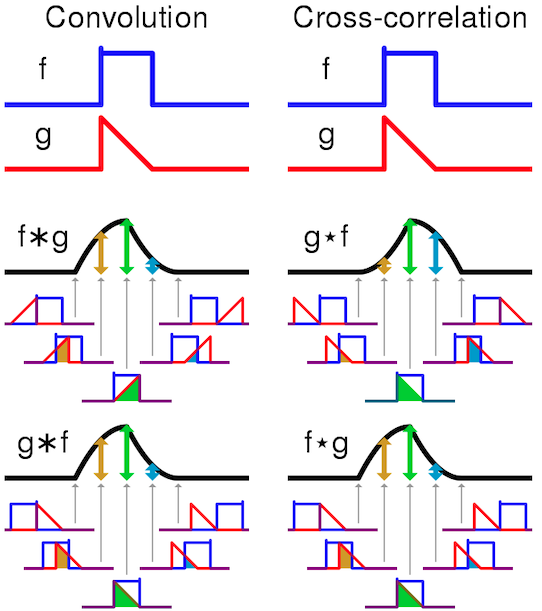
\includegraphics[width=0.99\textwidth]
            {./images/convolution/wikipedia_comparison_conv_corr_02.png}\\
         {\scriptsize 
          Comparison of convolution, cross-correlation.\\
          \color{col:attribution} 
          Image reproduced from \cite{Wikipedia:Convolution}}\\
          \end{center}
        \end{column}
        \begin{column}{0.55\textwidth}
            The \index{convolution}\gls{convolution} $(f \ast g) (x)$ of real-valued functions 
            $f(x)$ and $g(x)$ was defined in 
            Eqs. \ref{eq:convolution_cont1d_1} and \ref{eq:convolution_cont1d_2}.\\
            \vspace{0.2cm}
            % \begin{equation*}
            %     (f \ast g) (x) = 
            %       \int_{-\infty}^{+\infty} 
            %         f(\alpha) g(x-\alpha) d\alpha = 
            %       \int_{-\infty}^{+\infty} 
            %         f(x-\alpha) g(\alpha) d\alpha
            % \end{equation*}                
            A related mathematical operation of the 
            \index{cross-correlation}\gls{cross-correlation} $(f \star g) (x)$.\\
            \vspace{0.2cm}
            The \index{convolution}\gls{convolution} $(f \ast g) (x)$ differs from 
            \index{cross-correlation}\gls{cross-correlation} $(f \star g) (x)$
            in that, in \gls{convolution}, 
            either $f(x)$ and $g(x)$ are reflected about the y axis.\\
        \end{column}
    \end{columns}

    \framebreak

    Usually, we work with data where $x$ takes discrete values 
    and $f(x)$ is stored as an array.
    We can define a discrete \index{convolution}\gls{convolution} as:
    \begin{equation}
        (f \ast g) (i) = 
          \sum_{m} 
            f(m) g(i-m)
        \label{eq:convolution_disc1d_1}
    \end{equation}        

    Very often, our input data are multi-dimensional 
    and our definition of the \gls{convolution} operation needs to be extended accordingly.
    For example, for an image described by a two-dimensional array $f$,
    \gls{convolution} is defined as:
    \begin{equation}
        (f \ast g) (i,j) = 
          \sum_{m} \sum_{n} 
          f(m,n) g(i-m, j-n)
        \label{eq:convolution_disc2d_1}
    \end{equation}        

    In \index{convolutional neural network}\gls{cnn} literature,
    $f$ is often referred to as the input, 
    while $g$ is referred to as the kernel.

    \framebreak
   
    The discrete \index{convolution}\gls{convolution}
    of two-dimensional data was defined as:
    \begin{equation*}
        (f \ast g) (i,j) = 
          \sum_{m} \sum_{n}
          f(m,n) g(i-m, j-n)
        \label{eq:convolution_disc2d_1}
    \end{equation*}        

    Using the commutative property of the convolution, it can be rewritten as:
    \begin{equation}
        (f \ast g) (i,j) = 
          \sum_{m} \sum_{n}
          f(i-m,j-n) g(m, n)
        \label{eq:convolution_disc2d_2}
    \end{equation}        

    In practical applications, the latter expression 
    where the kernel $g$ is flipped relative to the input $f$ is easier to implement.
    \begin{itemize}
      \item The kernel has a smaller range than the input.\\
    \end{itemize}
    \vspace{0.2cm}

    Actually, many \gls{ml} libraries implement the following 
    \index{cross-correlation}\gls{cross-correlation}, but call it \gls{convolution}:
    \begin{equation}
        (f \star g) (i,j) = 
          \sum_{m} \sum_{n}
          f(i+m,j+n) g(m, n)
        \label{eq:cross_correlation_disc2d_1}
    \end{equation}        

    \framebreak

    \begin{center}
        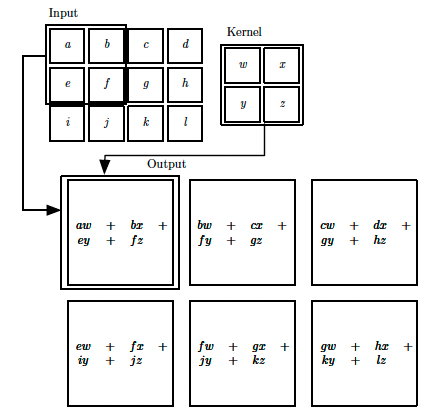
\includegraphics[width=0.60\textwidth]
        {./images/convolution/goodfellow17_convolution_2d_01.png}\\
     {\scriptsize 
      An example of 2-D convolution.\\
      \color{col:attribution} 
      Image reproduced from p.325 of \cite{Goodfellow:2017MITDL}}\\
    \end{center}

\end{frame}

